\subsection{Perceptron}
Perceptrons easily overfit

        \begin{center}
        \begin{tabular}{| c | c || c | c | c | c |}
        \hline
        Dataset & Label & Accuracy & f1 & Precision & Recall \\
        \hline \hline
         Training & Default         & 74.2\% & 19.4\% & 25.6\% & 15.5\% \\
         Training & Paid in Full    &       & 84.6\% & 80.9\% & 88.8\% \\
         \hline
         Test & Default             & 74.4\% & 19.8\% & 26.0\% & 16.0\% \\
         Test & Paid in Full        &       & 84.8\% & 81.2\% & 88.8\% \\
         \hline
        \end{tabular}
        \end{center}


\subsubsection{Logistic Regression}
Logistic Regression was surprisingly powerful, not surprising

        \begin{center}
        \begin{tabular}{| c | c || c | c | c | c |}
        \hline
        Dataset & Label & Accuracy & f1 & Precision & Recall \\
        \hline \hline
         Training & Default         & 80.3\% & 9.1\% & 55.3\% & 5.0\% \\
         Training & Paid in Full    &       & 88.9\% & 80.7\% & 99.0\% \\
         \hline
         Test & Default             & 80.5\% & 9.4\% & 55.1\% & 51.2\% \\
         Test & Paid in Full        &       & 89.1\% & 81.0\% & 99.0\% \\
         \hline
        \end{tabular}
        \end{center}


\subsubsection{Random Forests}

As expected, ensemble learning from decision trees quickly over-fits training data.

        \begin{center}
        \begin{tabular}{| c | c || c | c | c | c |}
        \hline
        Dataset & Label & Accuracy & f1 & Precision & Recall \\
        \hline \hline
         Training & Default         & 100.0\% & 100.0\% & 100.0\% & 100.0\% \\
         Training & Paid in Full    &       & 100.0\% & 100.0\% & 100.0\% \\
         \hline
         Test & Default             & 80.5\% & 12.7\% & 53.8\% & 7.2\% \\
         Test & Paid in Full        &       & 89.0\% & 81.2\% & 98.5\% \\
         \hline
        \end{tabular}
        \end{center}


\subsubsection{SVM}

        \begin{center}
        \begin{tabular}{| c | c || c | c | c | c |}
        \hline
        Dataset & Label & Accuracy & f1 & Precision & Recall \\
        \hline \hline
         Training & Default         & 80.1\% & 3.3\% & 50.5\% & 1.7\% \\
         Training & Paid in Full    &       & 88.9\% & 80.3\% & 99.6\% \\
         \hline
         Test & Default             & 80.3\% & 3.4\% & 48.7\% & 1.8\% \\
         Test & Paid in Full        &       & 89.0\% & 80.5\% & 99.5\% \\
         \hline
        \end{tabular}
        \end{center}


\subsubsection{Neural Net}

\begin{figure}[h!]
	\centering
	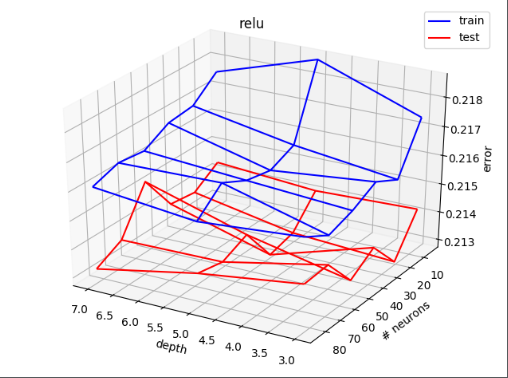
\includegraphics[width=10cm, height=7cm]{neural_nets.png}
	\caption{Train and Test Error for Various Architectures}
	\label{fig:neural_net}
\end{figure}

Not much variance or improvements with deeper models, best to keep it simple
